\documentclass[a4paper]{article}
\usepackage[italian]{babel}
\usepackage[utf8]{inputenc}
\usepackage[T1]{fontenc}
\usepackage{enumitem}
\usepackage{graphicx}
\usepackage{float}
\usepackage{longtable}
\usepackage[table]{xcolor}
\usepackage{geometry}

\usepackage{lastpage}
\usepackage[bottom]{footmisc}
\usepackage{fancyhdr}
\usepackage{tabu}

\usepackage{pgffor}
\usepackage{etoolbox}
\usepackage{multirow}



\usepackage[official]{eurosym}

% Navigazione pdf
\usepackage{hyperref}
\hypersetup{
	colorlinks=true,
	linkcolor=black,
	filecolor=magenta,      
	urlcolor=blue,
}

\usepackage{tabularx}

\usepackage{multicol}
\newcommand{\glo}{\textsubscript{\emph{G}}}
\newcommand\hd{\emph{HD Viz}}
\newcommand\cod{\emph{Code of Duty}}
\newcommand{\myparagraph}[1]{\paragraph{#1}\mbox{}\\}
\newcommand{\mysubparagraph}[1]{\subparagraph{#1}\mbox{}\\}

\newcommand{\NdP}{\emph{Norme di Progetto 3.0.0}}
\newcommand{\PdP}{\emph{Piano di Progetto 3.0.0}}
\newcommand{\AdR}{\emph{Analisi dei requisiti 3.0.0}}
\newcommand{\PdQ}{\emph{Piano di Qualifica 3.0.0}}

\definecolor{header}{HTML}{FA8D21}
\definecolor{pari}{HTML}{DBDBDB}
\definecolor{dispari}{HTML}{F5F5F5}

\setcounter{secnumdepth}{4}

\pagestyle{fancy}
\lhead{
\includegraphics[scale=0.06]{../_template/images/logo_crop.png}}

%Titolo del documento
\rhead{\titolodocumento{}}
\cfoot{Pagina \thepage\ di \pageref{LastPage}}
\renewcommand{\footrulewidth}{0.4pt}

\newcommand{\titolodocumento}{Analisi dei requisiti} % Titolo documento
\newcommand{\versione}{ 2.3.0 } % Versione documento
\newcommand{\approvazione}{ Diego Piola } % Responsabile di progetto
\newcommand{\redazione}{\parbox[t]{4cm} {Andrea Mascari\\Damiano Zanardo\\Diego Piola\\}} % Redattori di questo documento
\newcommand{\verifica}{\parbox[t]{4cm} {Andrea Mascari\\Damiano Zanardo \\ Diego Piola \\ Alessandro Flori \\ } } % Verificatori di questo documento
\newcommand{\stato}{In lavorazione} % Approvato 
\newcommand{\uso}{Esterno} % Interno - Esterno
\newcommand{\destinazione}{\parbox[t]{4cm}{Prof Tullio Vardanega \\ Prof. Riccardo Cardin} } % Destinatario ( D1\\D2\\D3 )
\newcommand{\descrizionedocumento}{Il documento elenca casi d'uso e requisiti del progetto } % Descrizione documento

% Mettere sempre la virgola dopo l'ultima riga, se no si rompe la tabella

\def\modifiche{
    {v0.0.1, 02/12/2020, Damiano Zanardo, Analista , Prima bozza{,} aggiunti tutti i capitolati},
}



% Per modificare il frontespizio e diario delle modifiche andare sulla cartella source
% Per aggiungere il contenuto andare sulla cartella source/sections e creare un nuovo file.tex per ogni sezione

% Per parole che devono andare nel glossario aggiungere /glo{} dopo la parola

\begin{document}
    % Frontespizio 
    %\documentclass[a4paper]{article}
%\usepackage[italian]{babel}
\usepackage[utf8]{inputenc}
\usepackage[T1]{fontenc}
\usepackage{enumitem}
\usepackage{graphicx}
\usepackage{float}
\usepackage{longtable}
\usepackage[table]{xcolor}
\usepackage{geometry}

\usepackage{lastpage}
\usepackage[bottom]{footmisc}
\usepackage{fancyhdr}
\usepackage{tabu}

\usepackage{pgffor}
\usepackage{etoolbox}
\usepackage{multirow}



\usepackage[official]{eurosym}

% Navigazione pdf
\usepackage{hyperref}
\hypersetup{
	colorlinks=true,
	linkcolor=black,
	filecolor=magenta,      
	urlcolor=blue,
}

\usepackage{tabularx}

\usepackage{multicol}
%\begin{document}

\begin{titlepage}

	\begin{center}
		
\includegraphics[scale = 0.5]{../_template/images/logo.png}\\
		\large \textbf{Code of Duty - Progetto \emph{HD VIZ}} \\
		\vfill
		\huge \textbf{\titolodocumento}
		\vspace*{\fill}
        
        \vfill
        \large
    \end{center}
    
	\begin{table}[htbp]
        \centering
        \begin{tabular}{r|l}
            \textbf{Versione} & \versione{} \\
            \textbf{Approvazione} & \approvazione{} \\
            \textbf{Redazione} & \redazione{} \\
            \textbf{Verifica} & \verifica{} \\
            \textbf{Stato} & \stato{} \\
            \textbf{Uso} & \uso{} \\
            \textbf{Destinato a} & \destinazione{}
        \end{tabular}
    \end{table}
    
    \begin{center}
        \vfill
        \normalsize
        \textbf{Descrizione}\\
		\descrizionedocumento
        \vfill
        \small
        \texttt{info@codeofduty.it}
	\end{center}
\end{titlepage}

%\end{document}

    
    % Diario delle modifiche
    \newcommand*\mytablecontents{}
\foreach \x [count=\nj] in \modifiche
{
    \foreach \y [count=\ni] in \x
    {
        \ifnum\ni=6
            \xappto\mytablecontents{\y}
            \gappto\mytablecontents{\\}
            \gappto\mytablecontents{\hline}
        \else
            \xappto\mytablecontents{\y&}
        \fi
    }
}

\section*{Diario delle modifiche}

% Impostazioni della tabella
\tabulinesep = 2mm % padding
\taburowcolors [1] 2{pari .. dispari} % colori delle righe
\begin{longtabu} to \textwidth {| X[0.3, c m] | X[0.6,c m] | X[0.7,c m] | X[0.9,c m] | X[0.7,c m] | X[1.2,l m]|} % larghezza delle colonne
\hline
\rowcolor{header} % colore dell'header

\textbf{Ver.} & \textbf{Data} & \textbf{Nominativo} & \textbf{Ruolo} & \textbf{Verificatore} & \multicolumn{1}{c|}{\textbf{Descrizione}}\\
\hline
\mytablecontents

\end{longtabu}

    \pagebreak
    
    % Indice
    \tableofcontents
    \pagebreak
    
    % Se necessari
    % \listoffigures
    \listoftables
    \pagebreak
    
    % Contenuto
    \section{Introduzione}
\subsection{Scopo del documento}
	In questo documento vengono illustrate le modalità con cui il gruppo \textit{Code of Duty} affronterà lo sviluppo del progetto \hd, quali:
	\begin{itemize}
    		\item Analisi dei rischi;
    		\item Presentazione del modello di sviluppo adottato;
    		\item Pianificazione delle attività e divisione dei ruoli;
    		\item Stima dei costi economici e risorse necessarie al compimento del progetto.
	\end{itemize}
\subsection{Scopo del prodotto}
	L'obiettivo del progetto è quello di creare un'applicazione di visualizzazione di dati con molte dimensioni. L'applicazione dovra permettere diverse visualizzazioni dei dati tramite browser ed è richiesta anche una parte server di supporto che permetta il prelevamento dei dati e la loro elaborazione.
\subsection{Glossario}
	In questo documento vengono definiti e descritti tutti i termini e tecnologie al fine di evitare ambiguità relative al linguaggio utilizzato nei documenti formali. Per facilitare la lettura i termini saranno contrassegnati da una 'G' a pedice.  
\subsection{Riferimenti}
	\subsubsection{Normativi}
		\begin{itemize}
			\item \textbf{Norme di Progetto}: \textit{Norme di progetto 2.0.0};
			\item \textbf{Regolamento organigramma e specifica tecnico-economica} : \href{https://www.math.unipd.it/~tullio/IS-1/2020/Progetto/RO.html}{RO}.
		\end{itemize}
	\subsubsection{Informativi}
		\begin{itemize}
			\item \textbf{Capitolato d'interesse}: \href{https://www.math.unipd.it/~tullio/IS-1/2020/Progetto/C4.pdf}{HD Viz - Visualizzazione di dati con molte dimensioni};
			\item \textbf{Il ciclo di vita del Software}: \href{https://www.math.unipd.it/~tullio/IS-1/2020/Dispense/L05.pdf}{L05};
			\item \textbf{Gestione di progetto}: \href{https://www.math.unipd.it/~tullio/IS-1/2020/Dispense/L06.pdf}{L06}.
		\end{itemize}
\subsection{Scadenze}
	Il gruppo \textit{Code of Duty} ha deciso di impegnarsi a rispettare le seguenti scadenze per lo sviluppo del progetto \hd
	\begin{itemize}
		\item \textbf{Revisione dei Requisiti}: 11-Gennaio-2021;
		\item \textbf{Revisione di Progettazione}: 10-Marzo-2021;
		\item \textbf{Revisione di Qualifica}: 2-Aprile-2021;
		\item \textbf{Revisione di Accettazione}: 3-Maggio-2021;
	\end{itemize}

    \section{Descrizione generale}
    \section{Casi d'uso}
    \subsection{Introduzione}
    In questa sezione vengono descritti i casi d'uso 
    \subsection{Attori}
    \begin{itemize}
        \item Utente
    \end{itemize}
    \subsection{UC1 - Inserimento dei dati }
\label{uc1}

    \begin{figure}[htbp]
        \centering
        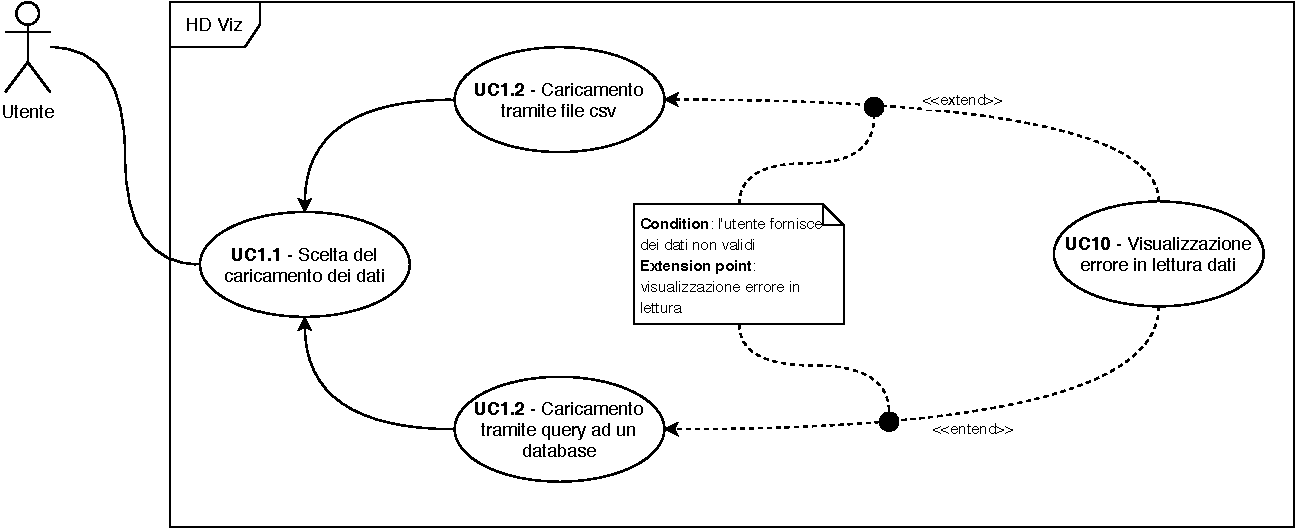
\includegraphics[width=1.0\textwidth]{source/sections/casi-uso/diagrams/uc1.pdf}
        \caption{UC1 - Inserimento dei dati}
        % \label{fig:uc1}
    \end{figure}
    
    \begin{itemize}
    \item \textbf{Attore}: utente;
    \item \textbf{Descrizione}: l'utente carica i dati per ottenere una visualizzazione;
    \item \textbf{Precondizione}:
    \begin{itemize}
        \item il sistema è funzionante e raggiungibile;
        \item l'utente accede alla pagina dell'applicazione.
    \end{itemize}
    \item \textbf{Postcondizione}: i dati sono stati caricati correttamente come matrice $N\times M$;
    \item \textbf{Scenario Principale}: 
        \begin{enumerate}
            \item l'utente accede alla pagina dell'applicazione;
            \item l'utente sceglie come caricare i dati (\hyperref[uc1.1]{UC1.1}):
                \begin{enumerate}
                    \item l'utente ha scelto di ricavare i dati caricando un file csv;
                    \item l'utente ha scelto di ricavare i dati tramite una query a un database.
                \end{enumerate}
        \end{enumerate}  
    \item \textbf{Estensioni}:
        \begin{enumerate}
            \item l'utente inserisce dei dati non validi o non nel formato corretto:
                \begin{enumerate}
                    \item fallisce l'inserimento dei dati;
                    \item viene visualizzato un messaggio di errore in lettura dei dati (\hyperref[uc10]{UC10}).
                \end{enumerate}
        \end{enumerate}  
    \item \textbf{Generalizzazioni}:
        \begin{enumerate}
            \item l'utente sceglie come caricare i dati:
                \begin{enumerate}
                    \item caricando un file csv (\hyperref[uc1.2]{UC1.2});
                    \item tramite una query a un database (\hyperref[uc1.3]{UC1.3}).
                \end{enumerate}
        \end{enumerate}  
    \end{itemize}
    
    %%%
    \subsubsection{UC1.1 - Scelta del caricamento dei dati}
    \label{uc1.1}
    
    \begin{itemize}
    \item \textbf{Attore}: utente;
    \item \textbf{Descrizione}: l'utente sceglie come caricare i dati;
    \item \textbf{Precondizione}:
    \begin{itemize}
        \item il sistema è funzionante e raggiungibile;
        \item l'utente accede alla pagina dell'applicazione.
    \end{itemize}
    \item \textbf{Postcondizione}: l'utente ha fatto la scelta;
    \item \textbf{Scenario Principale}: 
        \begin{enumerate}
            \item l'utente sceglie come caricare i dati in base alle proprie esigenze.
        \end{enumerate}
    \end{itemize}
    
    %%%
    \subsubsection{UC1.2 - Caricamento tramite file csv}
    \label{uc1.2}
    
    \begin{itemize}
    \item \textbf{Attore}: utente;
    \item \textbf{Descrizione}: l'utente sceglie di caricare i dati tramite un file csv;
    \item \textbf{Precondizione}:
    \begin{itemize}
        \item il sistema è funzionante e raggiungibile;
        \item l'utente accede alla pagina dell'applicazione;
        \item l'utente è in possesso di un file csv contenete i dati.
    \end{itemize}
    \item \textbf{Input}: file csv contenente i dati da visualizzare;
    \item \textbf{Postcondizione}: l'utente ha caricato il suo file csv come matrice $N\times M$;
    \item \textbf{Scenario Principale}: 
        \begin{enumerate}
            \item l'utente ha scelto di inserire i file tramite un file csv;
            \item tramite l'apposito bottone sceglie il file.
        \end{enumerate}
        \item \textbf{Estensioni}:
        \begin{enumerate}
            \item l'utente inserisce dei dati non validi o non nel formato corretto:
                \begin{enumerate}
                    \item fallisce l'inserimento dei dati;
                    \item viene visualizzato un messaggio di errore in lettura dei dati. (\hyperref[uc10]{UC10}):
                \end{enumerate}
        \end{enumerate}  
    \end{itemize}

    
    %%%
    \subsubsection{UC1.3 - Caricamento tramite query ad un database}
    \label{uc1.3}
    
    Il caricamento tramite database è descritto in modo generale. L'analisi più approfondita di questo requisito sarà stesa durante la prossima revisione, dopo aver fissato una \emph{Technology Baseline}. In ogni caso sarà possibile ricavare i dati da almeno un tipo di database SQL e da almeno un tipo di database NoSQL.
    
    \begin{itemize}
    \item \textbf{Attore}: utente;
    \item \textbf{Descrizione}: l'utente sceglie di caricare i dati tramite tramite query ad un database;
    \item \textbf{Precondizione}:
    \begin{itemize}
        \item il sistema è funzionante e raggiungibile;
        \item l'utente accede alla pagina dell'applicazione;
        \item l'utente può collegarsi ad un database (possiede le credenziali).
    \end{itemize}
    \item \textbf{Postcondizione}: l'utente si è collegato al database e ha recuperato i dati tramite query come matrice $N\times M$;
    \item \textbf{Scenario Principale}: 
        \begin{enumerate}
            \item l'utente ha scelto di caricare i dati tramite tramite query ad un database in cui può collegarsi;
            \item inserisce le credenziali, e scrive la sua query per ricavare i dati.
        \end{enumerate}
        \item \textbf{Estensioni}:
        \begin{enumerate}
            \item l'utente inserisce dei dati non validi o non nel formato corretto:
                \begin{enumerate}
                    \item fallisce l'inserimento dei dati;
                    \item viene visualizzato un messaggio di errore in lettura dei dati (\hyperref[uc10]{UC10}).
                \end{enumerate}
        \end{enumerate}  
    \end{itemize}

    
    \pagebreak
    \subsection{UC2 - Scelta della visualizzazione }
\label{uc2}

    % \includegraphics{}
    \begin{itemize}
    \item \textbf{Attore}: Utente
    \item \textbf{Descrizione}: L'utente all'interno dell'applicazione sceglie la visualizzazione che vuole ottenere
    \item \textbf{Precondizione}:
    \begin{itemize}
        \item Il sistema è funzionante e raggiungibile
        \item L'utente accede alla pagina dell'applicazione
    \end{itemize}
    \item \textbf{Postcondizione}: L'utente ha scelto quale visualizzazione vuole ottenere
    \item \textbf{Scenario Principale}: 
        \begin{enumerate}
            \item L'utente seleziona la visualizzazione tra quelle disponibili
        \end{enumerate}  
    \item \textbf{Generalizzazioni}:
        \begin{enumerate}
            \item L'utente seleziona una delle seguenti visualizzazioni
                \begin{enumerate}
                    \item Scatter Plot Matrix (\hyperref[uc2.1]{UC2.1})
                    \item Heatmap (\hyperref[uc2.2]{UC2.2})
                    \item Correlation Heatmap (\hyperref[uc2.3]{UC2.3})
                    \item Force Field (\hyperref[uc2.4]{UC2.4})
                    \item Linear Projection (\hyperref[uc2.5]{UC2.5})
                    \item Parallel Coordinates (\hyperref[uc2.6]{UC2.6})
                \end{enumerate}
        \end{enumerate}  
    \end{itemize}
    
    %%%
    \subsubsection{UC2.1 - Scatter Plot Matrix}
    \label{uc2.1}
    
    \begin{itemize}
    \item \textbf{Attore}: Utente
    \item \textbf{Descrizione}: L'utente sceglie la visualizzazione \emph{Scatter Plot Matrix}
    \item \textbf{Precondizione}:
    \begin{itemize}
        \item Il sistema è funzionante e raggiungibile
        \item L'utente accede alla pagina dell'applicazione
    \end{itemize}
    \item \textbf{Postcondizione}: L'utente sceglie Scatter Plot Matrix come visualizzazione
    \item \textbf{Scenario Principale}: 
        \begin{enumerate}
            \item L'utente sceglie Scatter Plot Matrix come visualizzazione
        \end{enumerate}
    \end{itemize}
    
    %%%
    \subsubsection{UC2.2 - Heatmap}
    \label{uc2.2}
    
    \begin{itemize}
    \item \textbf{Attore}: Utente
    \item \textbf{Descrizione}: L'utente sceglie la visualizzazione \emph{Heatmap}
    \item \textbf{Precondizione}:
    \begin{itemize}
        \item Il sistema è funzionante e raggiungibile
        \item L'utente accede alla pagina dell'applicazione
    \end{itemize}
    \item \textbf{Postcondizione}: L'utente sceglie Heatmap come visualizzazione
    \item \textbf{Scenario Principale}: 
        \begin{enumerate}
            \item L'utente sceglie Heatmap come visualizzazione
        \end{enumerate}
    \end{itemize}
    
    %%%
    \subsubsection{UC2.3 - Correlation Heatmap}
    \label{uc2.3}
    
    \begin{itemize}
    \item \textbf{Attore}: Utente
    \item \textbf{Descrizione}: L'utente sceglie la visualizzazione \emph{Correlation Heatmap}
    \item \textbf{Precondizione}:
    \begin{itemize}
        \item Il sistema è funzionante e raggiungibile
        \item L'utente accede alla pagina dell'applicazione
    \end{itemize}
    \item \textbf{Postcondizione}: L'utente sceglie Correlation Heatmap come visualizzazione
    \item \textbf{Scenario Principale}: 
        \begin{enumerate}
            \item L'utente sceglie Correlation Heatmap come visualizzazione
        \end{enumerate}
    \end{itemize}
    
    %%%
    \subsubsection{UC2.4 - Force Field}
    \label{uc2.4}
    
    \begin{itemize}
    \item \textbf{Attore}: Utente
    \item \textbf{Descrizione}: L'utente sceglie la visualizzazione \emph{Force Field}
    \item \textbf{Precondizione}:
    \begin{itemize}
        \item Il sistema è funzionante e raggiungibile
        \item L'utente accede alla pagina dell'applicazione
    \end{itemize}
    \item \textbf{Postcondizione}: L'utente sceglie Force Field come visualizzazione
    \item \textbf{Scenario Principale}: 
        \begin{enumerate}
            \item L'utente sceglie Force Field come visualizzazione
        \end{enumerate}
    \end{itemize}
    
    %%%
    \subsubsection{UC2.5 - Linear Projection}
    \label{uc2.5}
    
    \begin{itemize}
    \item \textbf{Attore}: Utente
    \item \textbf{Descrizione}: L'utente sceglie la visualizzazione \emph{Linear Projection}
    \item \textbf{Precondizione}:
    \begin{itemize}
        \item Il sistema è funzionante e raggiungibile
        \item L'utente accede alla pagina dell'applicazione
    \end{itemize}
    \item \textbf{Postcondizione}: L'utente sceglie Linear Projection come visualizzazione
    \item \textbf{Scenario Principale}: 
        \begin{enumerate}
            \item L'utente sceglie Linear Projection come visualizzazione
        \end{enumerate}
    \end{itemize}
    
    %%%
    \subsubsection{UC2.6 - Parallel Coordinates}
    \label{uc2.6}
    
    \begin{itemize}
    \item \textbf{Attore}: Utente
    \item \textbf{Descrizione}: L'utente sceglie la visualizzazione \emph{Parallel Coordinates}
    \item \textbf{Precondizione}:
    \begin{itemize}
        \item Il sistema è funzionante e raggiungibile
        \item L'utente accede alla pagina dell'applicazione
    \end{itemize}
    \item \textbf{Postcondizione}: L'utente sceglie Parallel Coordinates come visualizzazione
    \item \textbf{Scenario Principale}: 
        \begin{enumerate}
            \item L'utente sceglie Parallel Coordinatescome visualizzazione
        \end{enumerate}
    \end{itemize}
    
  

    \pagebreak
    \subsection{UC3 - Scelta delle Labels}
\label{uc3}

    \begin{figure}[htbp]
        \centering
        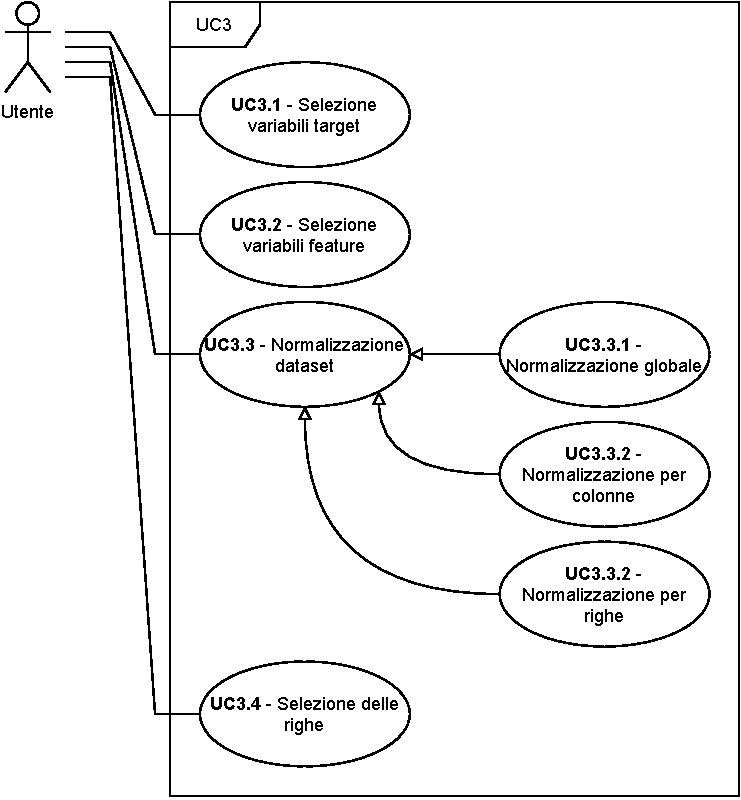
\includegraphics[width=0.5\textwidth]{source/sections/casi-uso/diagrams/uc3.pdf}
        \caption{UC3 - Scelta delle Labels}
        \label{fig:uc3}
    \end{figure}


    \begin{itemize}
    \item \textbf{Attore}: Utente
    \item \textbf{Descrizione}: Tra le dimensioni (colonne della matrice) del dataset caricato possono essere presenti delle labels, l'applicazione offre un meccanismo tramite cui l'utente può selezionare queste tipo di features e separarle dalle features numeriche che invece compongono le coordinate del dato $n$-dimensionale.
    \item \textbf{Precondizione}:
    \begin{itemize}
        \item Eseguito l'upload del dataset come matrice $N\times M$ (\hyperref[uc2]{UC2}).
        \item Selezionata una tra le visualizzazioni Scatter Plot Matrix (\hyperref[uc2.1]{UC2.1}), Force Field (\hyperref[uc2.4]{UC2.4}) Linear Projection (\hyperref[uc2.5]{UC2.5})
    \end{itemize}
    \item \textbf{Postcondizione}: Le features selezionate verranno considerate dal sistema come labels.
    \item \textbf{Scenario Principale}: 
    \begin{enumerate}
        \item L'utente visualizza le features del dataset.
        \item Seleziona le features del dato che ritiene essere delle labels.
    \end{enumerate}  
    \end{itemize}
    
    \subsubsection{UC3.1 - Assegnazione delle classi di visualizzazione alle Labels}
    \label{uc3.1}
    \begin{itemize}
    \item \textbf{Attore}: Utente
    \item \textbf{Descrizione}: L'utente decide di assegnare dei diversi modi per distinguere un punto nel grafico, assegnando una classe di visualizzazione (colore, forma, size) ad ogni label, in questo modo risulta più semplice per l'analista vedere dei pattern nella visualizzazione del grafico.
    \item \textbf{Precondizione}:
    \begin{itemize}
        \item Eseguito l'upload del dataset come matrice $N\times M$ (\hyperref[uc2]{UC2}).
        \item Selezionato una tra le visualizzazioni Scatter Plot Matrix (\hyperref[uc2.1]{UC2.1}), Force Field (\hyperref[uc2.4]{UC2.4}) Linear Projection (\hyperref[uc2.5]{UC2.5}).
        \item Nel dataset, almeno una feature è stata selezionata come label.
    \end{itemize}
    \item \textbf{Postcondizione}: Al variare del valore della etichetta $X$, i punti visualizzati assumono un diverso attributo della classe assegnata a quest'ultima.
    \item \textbf{Scenario Principale}: 
    \begin{enumerate}
        \item L'utente visualizza tutte le labels selezionate.
        \item L'utente associa ad ogni label una classe di visualizzazione.
    \end{enumerate}  
    \end{itemize}
    \pagebreak
    \subsection{UC4 - Selezione manuale delle Features}
\label{uc4}
 %   \includegraphics{}
    \begin{itemize}
    \item \textbf{Attore}: Utente
    \item \textbf{Descrizione}: L'utente può scartare le features di un dato che non è interessato a visualizzare.
    \item \textbf{Precondizione}: 
     \begin{itemize}
        \item Eseguito l'upload del dataset come matrice $N\times M$ (\hyperref[uc1]{UC1}).
        \item Selezionato un tipo di visualizzazione (\hyperref[uc2]{UC2}).
    \end{itemize}
    \item \textbf{Postcondizione}: La matrice contiene $M-i$ colonne, dove $i$ è il numero di features che l'utente ha scartato.
    \item \textbf{Scenario Principale}: 
    \begin{enumerate}
        \item L'utente visualizza le features del dataset, che corrispondono alle colonne della matrice
        \item L'utente scarta le features a cui non è interessato
    \end{enumerate}
    \item \textbf{Generalizzazioni}:
        \begin{enumerate}
            \item Selezione manuale delle features per Scatter Plot Matrix (\hyperref[uc4.1]{UC4.1})
        \end{enumerate}
    \end{itemize}
    
    \subsubsection{UC4.1 - Selezione manuale delle Features per Scatter Plot Matrix}
    \label{uc4.1}
    \begin{itemize}
    \item \textbf{Attore}: Utente
    \item \textbf{Descrizione}: L'utente può selezionare al massimo 5 features da visualizzare.
    \item \textbf{Precondizione}: 
     \begin{itemize}
        \item Eseguito l'upload del dataset come matrice $N\times M$ (\hyperref[uc1]{UC1}).
        \item Selezionato Scatter Plot Matrix come visualizzazione (\hyperref[uc2.1]{UC2.1}).
    \end{itemize}
    \item \textbf{Postcondizione}: La matrice contiene al massimo 5 colonne cioè le features che l'utente ha selezionato.
    \item \textbf{Scenario Principale}: 
    \begin{enumerate}
        \item L'utente visualizza le features del dataset, che corrispondono alle colonne della matrice
        \item L'utente sceglie le features che è intenzionato a visualizzare
    \end{enumerate}  
    \end{itemize}
    \pagebreak
    \subsection{UC5 - Calcolo matrice di distanza}
    \label{uc5}
    
    \begin{figure}[htbp]
        \centering
        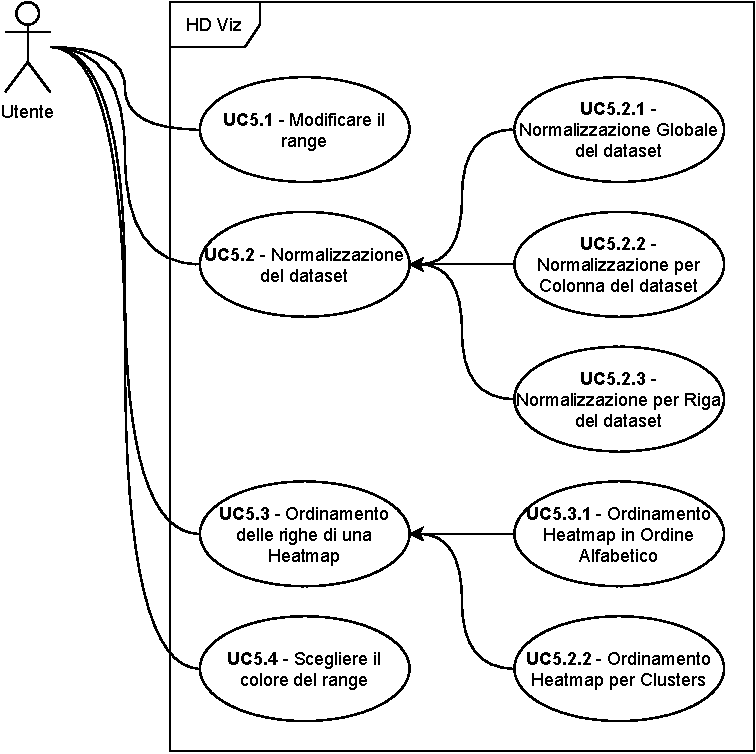
\includegraphics[width=0.9\textwidth]{source/sections/casi-uso/diagrams/uc5.pdf}
        \caption{UC5 - Calcolo matrice di distanza}
        \label{fig:uc5}
    \end{figure}
    
    \begin{itemize}
    \item \textbf{Attore}: utente;
    \item \textbf{Descrizione}: data una matrice $N \times M$ viene calcolata la distanza tra ogni riga e viene restituita all'utente una matrice di distanza N x N dove ${x_i}_j$ è la distanza tra la riga $i$ e la riga $j$ della matrice di partenza;
    \item \textbf{Precondizione}: 
    \begin{itemize}
        \item eseguito l'upload del dataset come matrice $N\times M$ (\hyperref[uc1.1]{UC1.1});
        \item selezionato Heatmap o Force Field come visualizzazione (\hyperref[uc2.1.2]{UC2.1.2} o \hyperref[uc2.1.4]{UC2.1.4}).
    \end{itemize}  
    \item \textbf{Postcondizione}: calcolata matrice di distanza $N \times N$ dove ${x_i}_j$ è la distanza tra la riga $i$ e la riga $j$ della matrice di partenza;
    \item \textbf{Scenario Principale}: 
    \begin{enumerate}
        \item l'utente seleziona il calcolo della matrice di distanza corrispondente al dataset caricato;
        \item l'utente seleziona la distanza (\hyperref[uc5.1]{UC5.1}).
    \end{enumerate}
    \end{itemize}
    
    \subsubsection{UC5.1 - Selezione distanza}
    \label{uc5.1}
    \begin{itemize}
    \item \textbf{Attore}: utente;
    \item \textbf{Descrizione}: l'utente sceglie la distanza da utilizzare per l'elaborazione del dataset;
    \item \textbf{Precondizione}: 
    \begin{itemize}
        \item eseguito l'upload del dataset come matrice $N\times M$ (\hyperref[uc1.1]{UC1.1}).
        \item selezionato Heatmap o Force Field come grafico su cui visualizzare il dataset (\hyperref[uc2.1.2]{UC2.1.2} o \hyperref[uc2.1.4]{UC2.1.4}).
        \item selezionato calcola matrice di distanza (\hyperref[uc5]{UC5}).
    \end{itemize}  
    \item \textbf{Postcondizione}: l'utente ha scelto la distanza da utilizzare;
    \item \textbf{Scenario Principale}: 
    \begin{enumerate}
        \item l'utente seleziona la distanza tra quelle disponibili.
    \end{enumerate}
    \item \textbf{Generalizzazioni}:
        \begin{enumerate}
            \item l'utente seleziona una delle seguenti distanze:
                \begin{enumerate}
                    \item Euclidea (\hyperref[uc5.1.1]{UC5.1.1});
                    \item Manhattan (\hyperref[uc5.1.2]{UC5.1.2}).
                \end{enumerate}
        \end{enumerate}  
    \end{itemize}
    
    \paragraph{UC5.1.1 - Distanza euclidea}
    \label{uc5.1.1}
    \begin{itemize}
    \item \textbf{Attore}: utente;
    \item \textbf{Descrizione}: l'utente sceglie la distanza \emph{Euclidea};
    \item \textbf{Precondizione}: 
    \begin{itemize}
        \item eseguito l'upload del dataset come matrice $N\times M$ (\hyperref[uc1.1]{UC1.1});
        \item selezionato Heatmap o Force Field come visualizzazione (\hyperref[uc2.1.2]{UC2.1.2} o \hyperref[uc2.1.4]{UC2.1.4}).
        \item selezionato calcola matrice di distanza (\hyperref[uc5]{UC5}).
    \end{itemize}  
    \item \textbf{Postcondizione}: l'utente ha scelto la distanza euclidea;
    \item \textbf{Scenario Principale}: 
    \begin{enumerate}
        \item l'utente ha scelto la distanza euclidea.
    \end{enumerate}
    \end{itemize}
    
    \paragraph{UC5.1.2 - Distanza di Manhattan}
    \label{uc5.1.2}
    \begin{itemize}
    \item \textbf{Attore}: utente;
    \item \textbf{Descrizione}: l'utente sceglie la distanza di \emph{Manhattan};
    \item \textbf{Precondizione}: 
    \begin{itemize}
        \item eseguito l'upload del dataset come matrice $N\times M$ (\hyperref[uc1.1]{UC1.1});
        \item selezionato Heatmap o Force Field come visualizzazione (\hyperref[uc2.1.2]{UC2.1.2} o \hyperref[uc2.1.4]{UC2.1.4}).
        \item selezionato calcola matrice di distanza (\hyperref[uc5]{UC5}).
    \end{itemize}  
    \item \textbf{Postcondizione}: l'utente ha scelto la distanza di Manhattan;
    \item \textbf{Scenario Principale}: 
    \begin{enumerate}
        \item l'utente ha scelto la distanza di Manhattan.
    \end{enumerate}
    \end{itemize}

    \pagebreak
        \subsection{UC6 - Calcolo Matrice di Distanza}
    % \includegraphics{}
    \begin{itemize}
    \item \textbf{Attore}: Utente
    \item \textbf{Descrizione}: Data una matrice $N \times M$ viene calcolata la distanza tra ogni riga e viene restituita all'utente una matrice di distanza N x N dove ${x_i}_j$ è la distanza tra la riga i e la riga j della matrice di partenza.
    \item \textbf{Precondizione}: 
    \begin{itemize}
        \item Eseguito l'upload del dataset come matrice $N\times M$ (\hyperref[uc1]{UC1}).
        \item Selezionato Heatmap o Force Field come visualizzazione (\hyperref[uc2.2]{UC2.2} o \hyperref[uc2.4]{UC2.4}).
    \end{itemize}  
    \item \textbf{Postcondizione}: Calcolata matrice di distanza $N \times N$ dove ${x_i}_j$ è la distanza tra la riga $i$ e la riga $j$ della matrice di partenza.
    \item \textbf{Scenario Principale}: 
    \begin{enumerate}
        \item L'utente seleziona il calcolo della matrice di distanza corrispondente al dataset caricato
        \item L'utente seleziona la distanza (\hyperref[uc6.1]{UC6.1})
    \end{enumerate}  
    \item \textbf{Inclusioni}:
        \begin{enumerate}
                \item \begin{enumerate}
                    \item Scelta dell'algoritmo di distanza da utilizzare (\hyperref[uc6.1]{UC6.1})
                \end{enumerate}
        \end{enumerate} 
    \end{itemize}
    
    \subsubsection{UC6.1 - Selezione distanza}
    \label{uc6.1}
    \begin{itemize}
    \item \textbf{Attore}: Utente
    \item \textbf{Descrizione}: L'utente sceglie la distanza da utilizzare durante l'elaborazione dati
    \item \textbf{Precondizione}: 
    \begin{itemize}
        \item Eseguito l'upload del dataset come matrice $N\times M$ (\hyperref[uc1]{UC1}).
        \item Selezionato Heatmap o Force Field come visualizzazione (\hyperref[uc2.2]{UC2.2} o \hyperref[uc2.4]{UC2.4}).
    \end{itemize}  
    \item \textbf{Postcondizione}: L'utente ha scelto la distanza da utilizzare
    \item \textbf{Scenario Principale}: 
    \begin{enumerate}
        \item L'utente seleziona la distanza tra quelle disponibili
    \end{enumerate}
    \item \textbf{Generalizzazioni}:
        \begin{enumerate}
            \item L'utente seleziona una delle seguenti distanze
                \begin{enumerate}
                    \item Euclidea (\hyperref[uc6.1.1]{UC6.1.1})
                    \item Manhattan (\hyperref[uc6.1.2]{UC6.1.2})
                \end{enumerate}
        \end{enumerate}  
    \end{itemize}
    
    \paragraph{UC6.1.1 - Distanza Euclidea}
    \label{uc6.1.1}
    \begin{itemize}
    \item \textbf{Attore}: Utente
    \item \textbf{Descrizione}: L'utente sceglie la distanza \emph{Euclidea}
    \item \textbf{Precondizione}: 
    \begin{itemize}
        \item Eseguito l'upload del dataset come matrice $N\times M$ (\hyperref[uc1]{UC1}).
        \item Selezionato Heatmap o Force Field come visualizzazione (\hyperref[uc2.2]{UC2.2} o \hyperref[uc2.4]{UC2.4}).
    \end{itemize}  
    \item \textbf{Postcondizione}: L'utente ha scelto la distanza euclidea
    \item \textbf{Scenario Principale}: 
    \begin{enumerate}
        \item L'utente ha scelto la distanza euclidea
    \end{enumerate}
    \end{itemize}
    
    \paragraph{UC6.1.2 - Distanza di Manhattan}
    \label{uc6.1.2}
    \begin{itemize}
    \item \textbf{Attore}: Utente
    \item \textbf{Descrizione}: L'utente sceglie la distanza di \emph{Manhattan}
    \item \textbf{Precondizione}: 
    \begin{itemize}
        \item Eseguito l'upload del dataset come matrice $N\times M$ (\hyperref[uc1]{UC1}).
        \item Selezionato Heatmap o Force Field come visualizzazione (\hyperref[uc2.2]{UC2.2} o \hyperref[uc2.4]{UC2.4}).
    \end{itemize}  
    \item \textbf{Postcondizione}: L'utente ha scelto la distanza di Manhattan
    \item \textbf{Scenario Principale}: 
    \begin{enumerate}
        \item L'utente ha scelto la distanza di Manhattan
    \end{enumerate}
    \end{itemize}
    \pagebreak
    \subsection{UC7 - Selezione algoritmo di riduzione delle componenti}
    \label{uc7}
    
    \begin{figure}[htbp]
        \centering
        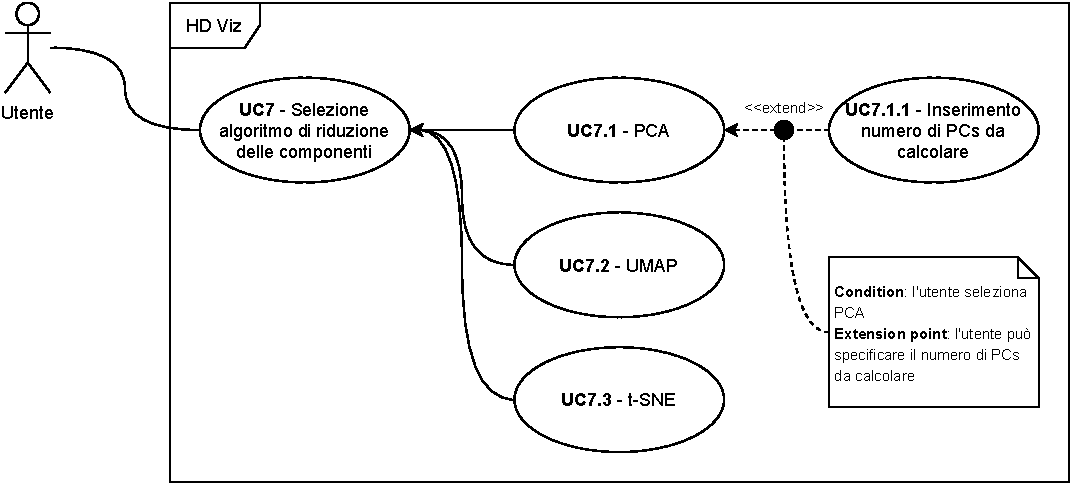
\includegraphics[width=0.9\textwidth]{source/sections/casi-uso/diagrams/uc7.pdf}
        \caption{UC7 - Selezione algoritmo di riduzione delle componenti}
        \label{fig:uc7}
    \end{figure}
    
    \begin{itemize}
    \item \textbf{Attore}: utente;
    \item \textbf{Descrizione}: l'utente sceglie l'algoritmo per la riduzione delle componenti per l'elaborazione dati;
    \item \textbf{Precondizione}: 
    \begin{itemize}
        \item eseguito l'upload del dataset come matrice $N\times M$ (\hyperref[uc1]{UC1});
        \item selezionato Linear Projection come visualizzazione \hyperref[uc2.5]{UC2.5}).
    \end{itemize}  
    \item \textbf{Postcondizione}: l'utente ha scelto l'algoritmo per la riduzione delle componenti;
    \item \textbf{Scenario Principale}: 
    \begin{enumerate}
        \item l'utente seleziona l'algoritmo per la riduzione delle componenti tra quelli disponibili.
    \end{enumerate}
    \item \textbf{Generalizzazioni}:
        \begin{enumerate}
            \item l'utente seleziona una delle seguenti distanze:
                \begin{enumerate}
                    \item PCA (\hyperref[uc7.1]{UC7.1});
                    \item UMAP (\hyperref[uc7.2]{UC7.2});
                    \item t-SNE (\hyperref[uc7.3]{UC7.3}).
                \end{enumerate}
        \end{enumerate}  
    \end{itemize}
    
    \subsubsection{UC7.1 - PCA}
    \label{uc7.1}
    \begin{itemize}
    \item \textbf{Attore}: utente;
    \item \textbf{Descrizione}: il PCA è una tecnica di riduzione dimensionale, cioè a partire da $n$ features ne calcola $k$ ($k$ fissato), queste nuove k feature approssimano meglio le $n$ features iniziali;
    \item \textbf{Precondizione}: 
    \begin{itemize}
        \item eseguito l'upload del dataset come matrice $N\times M$ (\hyperref[uc1]{UC1});
        \item selezionato Linear Projection come visualizzazione (\hyperref[uc2.5]{UC2.5}).
    \end{itemize}  
    \item \textbf{Postcondizione}: il dataset contiene k nuove colonne (dove $k$ è il numero di PCs che l'utente ha scelto di calcolare), che sono le $k$ proiezioni calcolate da PCA;
    \item \textbf{Scenario Principale}: 
    \begin{enumerate}
        \item l'utente sceglie di applicare l'algoritmo PCA sul dataset.
    \end{enumerate}  
    \item \textbf{Inclusioni}:
        \begin{enumerate}
            \item inserimento del numero di PCs da calcolare (\hyperref[uc7.1.1]{UC7.1.1}).
        \end{enumerate} 
    \end{itemize}
    
    \paragraph{UC7.1.1 - PCA - Inserimento numero di PCs da calcolare}
    \label{uc7.1.1}
    \begin{itemize}
    \item \textbf{Attore}: utente;
    \item \textbf{Descrizione}: l'utente specifica quante nuove features il PCA deve calcolare;
    \item \textbf{Precondizione}: 
    \begin{itemize}
        \item eseguito l'upload del dataset come matrice $N\times M$ (\hyperref[uc1]{UC1});
        \item selezionato Linear Projection come visualizzazione (\hyperref[uc2.5]{UC2.5});
        \item selezionato PCA (\hyperref[uc7.1]{UC7.1}).
    \end{itemize}  
    \item \textbf{Postcondizione}: il numero k di features da calcolare è stato inserito;
    \item \textbf{Scenario Principale}: 
    \begin{enumerate}
        \item l'utente inserisce un numero k compreso tra 1 e il numero di features.
    \end{enumerate}  
    \end{itemize}
    
    \subsubsection{UC7.2 - UMAP}
    \label{uc7.2}
    \begin{itemize}
    \item \textbf{Attore}: utente;
    \item \textbf{Descrizione}: UMAP è una tecnica di riduzione dimensionale, cioè a partire da $n$ features ne calcola $k$ ($k$ fissato), queste nuove k feature approssimano meglio le $n$ features iniziali;
    \item \textbf{Precondizione}: 
    \begin{itemize}
        \item eseguito l'upload del dataset come matrice $N\times M$ (\hyperref[uc1]{UC1});
        \item selezionato Linear Projection come visualizzazione (\hyperref[uc2.5]{UC2.5}).
    \end{itemize}  
    \item \textbf{Postcondizione}: l'utente seleziona UMAP come algoritmo per la riduzione dimensionale;
    \item \textbf{Scenario Principale}: 
    \begin{enumerate}
        \item l'utente sceglie di applicare l'algoritmo UMAP sul dataset.
    \end{enumerate}
    \end{itemize}
    
    \subsubsection{UC7.3 - t-SNE}
    \label{uc7.3}
    \begin{itemize}
    \item \textbf{Attore}: utente;
    \item \textbf{Descrizione}: t-SNE è una tecnica di riduzione dimensionale, cioè a partire da $n$ features ne calcola $k$ ($k$ fissato), queste nuove k feature approssimano meglio le $n$ features iniziali;
    \item \textbf{Precondizione}: 
    \begin{itemize}
        \item eseguito l'upload del dataset come matrice $N\times M$ (\hyperref[uc1]{UC1});
        \item selezionato Linear Projection come visualizzazione (\hyperref[uc2.5]{UC2.5}).
    \end{itemize}  
    \item \textbf{Postcondizione}: l'utente seleziona t-SNE come algoritmo per la riduzione dimensionale;
    \item \textbf{Scenario Principale}: 
    \begin{enumerate}
        \item l'utente sceglie di applicare l'algoritmo t-SNE sul dataset.
    \end{enumerate}
    \end{itemize}
    
    

    \pagebreak
    \subsection{UC8 - Elaborazione dati}
    \label{uc8}
    \begin{itemize}
    \item \textbf{Attore}: Utente
    \item \textbf{Descrizione}: Vengono elaborati i dati secondo le impostazioni
    \item \textbf{Precondizione}: 
    \begin{itemize}
        \item Eseguito l'upload del dataset come matrice $N\times M$ (\hyperref[uc1]{UC1}).
        \item Selezionato un tipo di visualizzazione (\hyperref[uc2]{UC2}).
    \end{itemize}  
    \item \textbf{Postcondizione}: L'applicazione dopo che l'utente ha caricato il suo dataset e selezionato il tipo di visualizzazione, ha elaborato i dati secondo le impostazioni
    \item \textbf{Scenario Principale}: 
    \begin{enumerate}
        \item L'utente carica il suo dataset (\hyperref[uc1]{UC1})
        \item L'utente seleziona il tipo di visualizzazione tra quelle disponibili (\hyperref[uc2]{UC2})
        \item L'applicazione elabora i dati con impostazioni di default (\hyperref[uc8.1]{UC8.1})
        \item L'utente cambia le impostazioni (\hyperref[uc3]{UC3} o \hyperref[uc4]{UC4} \hyperref[uc5]{UC5} o \hyperref[uc6]{UC6} o \hyperref[uc7]{UC7})
        \item L'applicazione rielabora i dati (\hyperref[uc8.2]{UC8.2})
    \end{enumerate}
    \end{itemize}
    
    % Nel caso di visualizzazioni che richiedono delle impostazioni obbligatorie? (esempio calcolare matrice di distanza prima di visualizzare il grafico force-field)
    \subsubsection{UC8.1 - Avvio elaborazione dati con impostazioni di default}
    \label{uc8.1}
    \begin{itemize}
    \item \textbf{Attore}: Utente
    \item \textbf{Descrizione}: L'utente avvia l'elaborazione dati secondo le impostazioni di deafult
    \item \textbf{Precondizione}: 
    \begin{itemize}
        \item Eseguito l'upload del dataset come matrice $N\times M$ (\hyperref[uc1]{UC1}).
        \item Selezionato un tipo di visualizzazione (\hyperref[uc2]{UC2}).
    \end{itemize}  
    \item \textbf{Postcondizione}: L'applicazione dopo che l'utente dopo ha caricato il suo dataset e selezionato il tipo di visualizzazione, ha avviato l'elaborazione dei dati secondo le impostazioni di default
    \item \textbf{Scenario Principale}: 
    \begin{enumerate}
        \item L'utente carica il suo dataset (\hyperref[uc1]{UC1})
        \item L'utente seleziona il tipo di visualizzazione tra quelle disponibili (\hyperref[uc2]{UC2})
        \item L'applicazione elabora i dati
    \end{enumerate}
    \end{itemize}
    
    \subsubsection{UC8.2 - Avvio elaborazione dati con impostazioni utente}
    \label{uc8.2}
    \begin{itemize}
    \item \textbf{Attore}: Utente
    \item \textbf{Descrizione}:  L'utente avvia l'elaborazione dati secondo le impostazioni personalizzate
    \item \textbf{Precondizione}: 
    \begin{itemize}
        \item Eseguito l'upload del dataset come matrice $N\times M$ (\hyperref[uc1]{UC1}).
        \item Selezionato un tipo di visualizzazione (\hyperref[uc2]{UC2}).
        \item L'utente ha cambiato le impostazioni (\hyperref[uc3]{UC3} o \hyperref[uc4]{UC4} \hyperref[uc5]{UC5} o \hyperref[uc6]{UC6} o \hyperref[uc7]{UC7})
    \end{itemize}  
    \item \textbf{Postcondizione}: L'applicazione dopo che l'utente ha caricato il suo dataset e selezionato il tipo di visualizzazione, ha avviato l'elaborazione dei dati secondo le impostazioni personalizzate inserite dall'utente
    \item \textbf{Scenario Principale}: 
    \begin{enumerate}
        \item L'utente carica il suo dataset (\hyperref[uc1]{UC1})
        \item L'utente seleziona il tipo di visualizzazione tra quelle disponibili (\hyperref[uc2]{UC2})
        \item L'applicazione elabora i dati (\hyperref[uc8.1]{UC8.1})
        \item L'utente cambia le impostazioni (\hyperref[uc3]{UC3} o \hyperref[uc4]{UC4} \hyperref[uc5]{UC5} o \hyperref[uc6]{UC6} o \hyperref[uc7]{UC7})
        \item L'applicazione rielabora i dati
    \end{enumerate}
    \end{itemize}
    \pagebreak
    \subsection{UC9 - Visualizzazione dati}
    \label{uc9}
    
    \begin{figure}[htbp]
        \centering
        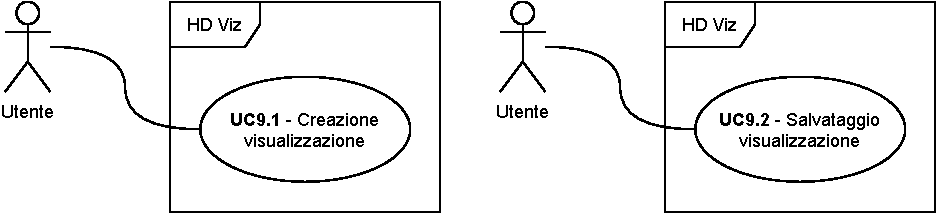
\includegraphics[width=0.9\textwidth]{source/sections/casi-uso/diagrams/uc9.pdf}
        \caption{UC9 - Visualizzazione dati}
        \label{fig:uc9}
    \end{figure}
    
    \begin{itemize}
    \item \textbf{Attore}: Utente
    \item \textbf{Descrizione}: L'utente avvia la visualizzazione del suo dataset secondo le impostazioni
    \item \textbf{Precondizione}: 
    \begin{itemize}
        \item Eseguito l'upload del dataset come matrice $N\times M$ (\hyperref[uc1]{UC1}).
        \item Selezionato un tipo di visualizzazione (\hyperref[uc2]{UC2}).
        \item Dati elaborati (\hyperref[uc8]{UC8})
    \end{itemize}  
    \item \textbf{Postcondizione}: L'applicazione dopo che l'utente dopo ha caricato il suo dataset e selezionato il tipo di visualizzazione, crea la visualizzazione richiesta sul dataset caricato
    \item \textbf{Scenario Principale}: 
    \begin{enumerate}
        \item L'utente carica il suo dataset (\hyperref[uc1]{UC1})
        \item L'utente seleziona il tipo di visualizzazione tra quelle disponibili (\hyperref[uc2]{UC2})
        \item L'applicazione elabora i dati (\hyperref[uc8]{UC8})
        \item L'applicazione crea la visualizzazione (\hyperref[uc9.1]{UC9.1})
        \item L'utente salva la visualizzazione (\hyperref[uc9.2]{UC9.2})
    \end{enumerate}
    \end{itemize}
    
    \subsubsection{UC9.1 - Creazione visualizzazione}
    \label{uc9.1}
    \begin{itemize}
    \item \textbf{Attore}: Utente
    \item \textbf{Descrizione}:  L'utente avvia la creazione della visualizzazione
    \item \textbf{Precondizione}: 
    \begin{itemize}
        \item Eseguito l'upload del dataset come matrice $N\times M$ (\hyperref[uc1]{UC1}).
        \item Selezionato un tipo di visualizzazione (\hyperref[uc2]{UC2}).
        \item Dati elaborati (\hyperref[uc8]{UC8})
    \end{itemize}  
    \item \textbf{Postcondizione}: L'applicazione dopo che l'utente dopo ha caricato il suo dataset e selezionato il tipo di visualizzazione, crea la visualizzazione a partire dai dati elaborati
    \item \textbf{Scenario Principale}: 
    \begin{enumerate}
        \item L'utente carica il suo dataset (\hyperref[uc1]{UC1})
        \item L'utente seleziona il tipo di visualizzazione tra quelle disponibili (\hyperref[uc2]{UC2})
        \item L'applicazione elabora i dati (\hyperref[uc8]{UC8})
        \item L'applicazione crea la visualizzazione
    \end{enumerate}
    \end{itemize}
    
    \subsubsection{UC9.2 - Salvataggio visualizzazione}
    \label{uc9.2}
    \begin{itemize}
    \item \textbf{Attore}: Utente
    \item \textbf{Descrizione}:  L'utente salva la visualizzazione
    \item \textbf{Precondizione}: 
    \begin{itemize}
        \item Eseguito l'upload del dataset come matrice $N\times M$ (\hyperref[uc1]{UC1}).
        \item Selezionato un tipo di visualizzazione (\hyperref[uc2]{UC2}).
        \item Dati elaborati (\hyperref[uc8]{UC8})
        \item Visualizzazione creata (\hyperref[uc9.1]{UC9.1})
    \end{itemize}  
    \item \textbf{Postcondizione}: L'utente ha salvato la visualizzazione come file immagine PNG
    \item \textbf{Output}: File PNG con la visualizzazione richiesta
    \item \textbf{Scenario Principale}: 
    \begin{enumerate}
        \item L'utente carica il suo dataset (\hyperref[uc1]{UC1})
        \item L'utente seleziona il tipo di visualizzazione tra quelle disponibili (\hyperref[uc2]{UC2})
        \item L'applicazione elabora i dati (\hyperref[uc8]{UC8})
        \item L'applicazione crea la visualizzazione
        \item L'utente salva (cliccando sul pulsante salva) la visualizzazione in formato PNG
    \end{enumerate}
    \end{itemize}
    \pagebreak
    \subsection{UC10 - Visualizzazione errore in lettura dati}
    \label{uc10}
    \begin{itemize}
    \item \textbf{Attore}: Utente
    \item \textbf{Descrizione}: L’utente visualizza un messaggio di errore dopo aver caricato un file non corretto o aver richiesto una query non corretta
    \item \textbf{Precondizione}: 
    \begin{itemize}
        \item L'utente fornisce un file non corretto o una query non corretta (\hyperref[uc1.2]{UC1.2} \hyperref[uc1.3]{UC1.3}).
    \end{itemize}  
    \item \textbf{Postcondizione}: Viene visualizzato un messaggio di errore e il caricamento dei dati fallisce
    \item \textbf{Scenario Principale}: 
    \begin{enumerate}
        \item Il caricamento dei dati fallisce
        \item Viene visualizzato il messaggio di errore
        \item L'utente clicca la X per chiudere il messaggio
    \end{enumerate}
    \end{itemize}
    \section{Requisiti}

    \subsection{Introduzione}
    La struttura dei requisiti è descritta nelle \emph{Norme di progetto}. Di seguito saranno elencati tutti i requisiti individuati dal gruppo. 
    
    \subsection{Requisiti funzionali}

\def\obb{Obbligatorio}

\def\requisitif{
    {RFO1, L'utente deve poter caricare i propri dati per la visualizzazione, \obb,Capitolato UC1},
    {RFO1.1, L'utente deve poter caricare i propri dati per la visualizzazione tramite file csv, \obb,Capitolato UC1.2},
    {RFO1.2, L'utente deve poter caricare i propri dati per la visualizzazione tramite query ad un database, \obb,Capitolato UC1.3},
    {RFO1.3, Il sistema deve visualizzare un messaggio di errore quando i dati caricati non sono corretti o è fallito un caricamento, \obb,Interno UC10},
    {RFO1.4, I dati caricati dovranno essere convertiti in JSON per uniformare l'elaborazione e la visualizzazione dei dati provenienti da fonti diverse, \obb, Interno},
    {RFO2, L'utente deve poter scegliere il tipo di visualizzazione, \obb,Capitolato UC2},
    {RFO2.1, L'utente deve poter scegliere Scatter Plot Matrix come tipo di visualizzazione, \obb,Capitolato UC2.1},
    {RFO2.2, L'utente deve poter scegliere Heatmap come tipo di visualizzazione, \obb,Capitolato UC2.2},
    {RFO2.2.1, L'utente deve poter scegliere il colore della sfumatura dell'Heatmap, \obb, UC5.4},
    {RFF2.3, L'utente deve poter scegliere Correlation Heatmap come tipo di visualizzazione, Facoltativo,Capitolato Interno UC2.3},
    {RFO2.4, L'utente deve poter scegliere Force Field come tipo di visualizzazione, \obb,Capitolato UC2.4},
    {RFO2.5, L'utente deve poter scegliere Linear Projection come tipo di visualizzazione, \obb,Capitolato UC2.5},
    {RFF2.6, L'utente deve poter scegliere Parallel Coordinates come tipo di visualizzazione, Facoltativo,Capitolato Interno UC2.6},
    {RFO3, L'utente deve poter scegliere le labels presenti nel suo dataset, \obb,Interno UC3},
    {RFO3.1, L'utente deve poter scegliere come visualizzare le labels presenti nel suo dataset all'interno della visualizzazione, \obb, Interno UC3.1},
    {RFO4, L'utente deve poter scartare le features di cui non è interessato o riaggiungere quelle scartate, \obb, Interno UC4},
    {RFO5, L'utente{,} se ha selezionato l'Heatmap{,} deve poter modificare le impostazioni che influenzano la visualizzazione, \obb,Interno UC5},
    {RFO5.1, L'utente se ha selezionato l'Heatmap deve poter modificare il range dei dati da considerare, \obb, Interno UC5.1},
    {RFO5.2, L'utente{,} se ha selezionato l'Heatmap{,} deve poter normalizzare il dataset, \obb,Interno UC5.2},
    {RFO5.2.1, L'utente deve poter normalizzare il dataset in modo globale, \obb, Interno UC5.2.1},
    {RFO5.2.2, L'utente deve poter normalizzare il dataset per colonna, \obb, Interno UC5.2.2},
    {RFO5.2.3, L'utente deve poter normalizzare il dataset per riga, \obb, Interno UC5.2.3},
    {RFO5.3, L'utente{,} se ha selezionato l'Heatmap{,} deve poter ordinare il dataset, \obb,Interno UC5.2},
    {RFO5.3.1, L'utente{,} se ha selezionato l'Heatmap{,} deve poter ordinare il dataset in ordine alfabetico, \obb,Interno UC5.3.1},
    {RFO5.3.2, L'utente{,} se ha selezionato l'Heatmap{,} deve poter ordinare il dataset in cluster, \obb,Capitolato UC5.3.2},
    {RFO5.4, L'utente se ha selezionato l'Heatmap deve poter assegnare un colore al range , \obb, Interno UC5.4},
    {RFO6, L'utente{,} se ha selezionato l'Heatmap{,} deve poter scegliere se utilizzare una matrice di distanza, \obb,Capitolato Interno UC6},
    {RFF6.1, L'utente{,} se ha selezionato l'Heatmap o il Force Field{,} deve poter scegliere quale funzione di distanza utilizzare, Facoltativo,Capitolato UC6.1},
    {RFF6.1.1, L'utente{,} se ha selezionato l'Heatmap o il Force Field{,} deve poter scegliere la distanza euclidea, Facoltativo,Interno UC6.1.1},
    {RFF6.1.2, L'utente{,} se ha selezionato l'Heatmap o il Force Field{,} deve poter scegliere la distanza di Manhattan, Facoltativo,Interno UC6.1.2},
    {RFO7, L'utente{,} se ha selezionato la Linear Projection{,} deve poter scegliere l'algoritmo per la riduzione delle componenti per l'elaborazione dati, \obb,Capitolato UC7},
    {RFF7.1, L'utente{,} se ha selezionato la Linear Projection{,} deve poter scegliere PCA come algoritmo per la riduzione delle componenti, Facoltativo,Interno UC7.1},
    {RFF7.2, L'utente{,} se ha selezionato la Linear Projection{,} deve poter scegliere UMAP come algoritmo per la riduzione delle componenti, Facoltativo,Capitolato UC7.2},
    {RFF7.3, L'utente{,} se ha selezionato la Linear Projection{,} deve poter scegliere t-SNE come algoritmo per la riduzione delle componenti, Facoltativo,Capitolato UC7.3},
    {RFO8.1, Il sistema deve elaborare i dati con le impostazioni di default, \obb,Interno UC8.1},
    {RFO8.2, Il sistema deve elaborare i dati con le impostazioni personalizzate dall'utente, \obb,Interno UC8.2},
    {RFO9, L'utente deve poter visualizzare la visualizzazione creata dal sistema, \obb,Capitolato UC9{,} UC9.1},
    {RFO9.2, L'utente deve salvare la visualizzazione come file PNG, \obb, Interno UC9.2},
    {RFO10, L'utente visualizza un messaggio di errore se carica i files scorrettamente, \obb, Interno UC10},
}






    % {RFO1.2, L'utente deve poter caricare i propri dati per la visualizzazione tramite query ad un database, \obb, \hyperref[uc1.3]{UC1.3}},
    % {RFO1.3, Il sistema deve visualizzare un messaggio di errore quando i dati caricati non sono corretti o è fallito un caricamento, \obb, \hyperref[uc10]{UC10}},
    % {RFO1.4, I dati caricati dovranno essere convertiti in JSON per uniformare l'elaborazione e la visualizzazione dei dati provenienti da fonti diverse, \obb, Decisione interna},
    % {RFO2, L'utente deve poter scegliere il tipo di visualizzazione, \obb, \hyperref[uc2]{UC2}},
    % {RFO2.1, L'utente deve poter scegliere Scatter Plot Matrix come tipo di visualizzazione, \obb, \hyperref[uc2.1]{UC2.1}},
    % {RFO2.2, L'utente deve poter scegliere Heatmap come tipo di visualizzazione, \obb, \hyperref[uc2.2]{UC2.2}},
    % {RFO2.2.1, L'utente deve poter scegliere il colore della sfumatura dell'Heatmap, \obb, \hyperref[uc2.7]{UC2.7}},
    % {RFF2.3, L'utente deve poter scegliere Correlation Heatmap come tipo di visualizzazione, Facoltativo, \hyperref[uc2.3]{UC2.3}},
    % {RFO2.4, L'utente deve poter scegliere Force Field come tipo di visualizzazione, \obb, \hyperref[uc2.4]{UC2.4}},
    % {RFO2.5, L'utente deve poter scegliere Linear Projection come tipo di visualizzazione, \obb, \hyperref[uc2.5]{UC2.5}},
    % {RFF2.6, L'utente deve poter scegliere Parallel Coordinates come tipo di visualizzazione, Facoltativo, \hyperref[uc2.6]{UC2.6}},
    % {RFO3, L'utente deve poter scegliere le etichette presenti nel suo dataset, \obb, \hyperref[uc3]{UC3}},
    % {RFO3.1, L'utente deve poter scegliere come visualizzare le etichette presenti nel suo dataset all'interno della visualizzazione, \obb, \hyperref[uc3.1]{UC3.1}},



%%%
%%%
%%%
\newcommand*\requisitiftable{}
\foreach \x [count=\nj] in \requisitif
{
    \foreach \y [count=\ni] in \x
    {
        \ifnum\ni=4
            \xappto\requisitiftable{\y}
            \gappto\requisitiftable{\\}
            \gappto\requisitiftable{\hline}
        \else
            \xappto\requisitiftable{\y & }
        \fi
    }
}

%\subsection{Requisiti funzionali}

% Impostazioni della tabella
\tabulinesep = 2mm % padding
\taburowcolors [1] 2{pari .. dispari} % colori delle righe
\addcontentsline{lot}{table}{Requisiti funzionali}
\begin{longtabu} to \textwidth {| X[0.2 l m] | X[0.4 l m] |  X[0.2 l m] | X[0.2 l m] |} % larghezza delle colonne
\hline
\rowcolor{header} % colore dell'header
    
\textbf{Requisito} & \textbf{Descrizione} & \textbf{Classificazione} & \textbf{Fonte} \\
\hline
\requisitiftable

\end{longtabu}
    \subsection{Requisiti di qualità}

\def\obb{Obbligatorio}
\def\pdq{Piano di Qualifica}

%startTable
\def\requisitiq{
    {RQO1, Deve essere prodotto un manuale d'uso per l'utente, \obb, Capitolato},
    {RQO2, Deve essere prodotto un manuale manutentore, \obb, Capitolato},
    {RQD3, Il codice deve essere pubblicato su un repository pubblico, Desiderabile, Capitolato},
    {RQO4, Il codice deve seguire le norme di stile specificate nel documento Norme di Progetto, \obb, Interno{,} Norme di Progetto 1.0.0},
    {RQO5, Nella codifica{,} deve essere evitato l'utilizzo di chiamate ricorsive se non in casi strettamente necessari, \obb, Interno{,} Norme di Progetto 1.0.0},
}
%endTable





%%%
%%%
%%%
\newcommand*\requisitiqtable{}
\foreach \x [count=\nj] in \requisitiq
{
    \foreach \y [count=\ni] in \x
    {
        \ifnum\ni=4
            \xappto\requisitiqtable{\y}
            \gappto\requisitiqtable{\\}
            \gappto\requisitiqtable{\hline}
        \else
            \xappto\requisitiqtable{\y & }
        \fi
    }
}

%\subsection{Requisiti funzionali}

% Impostazioni della tabella
\tabulinesep = 2mm % padding
\taburowcolors [1] 2{pari .. dispari} % colori delle righe
\addcontentsline{lot}{table}{Requisiti di qualità}
\begin{longtabu} to \textwidth {| X[0.2 l m] | X[0.4 l m] |  X[0.2 l m] | X[0.2 l m] |} % larghezza delle colonne
\hline
\rowcolor{header} % colore dell'header
    
\textbf{Requisito} & \textbf{Descrizione} & \textbf{Classificazione} & \textbf{Fonte} \\
\hline
\requisitiqtable

\end{longtabu}
    \subsection{Requisiti di vincolo}

\def\obb{Obbligatorio}

%startTable
\def\requisitiv{
    {RVO1, Il codice sorgente dell'applicazione essere open source, \obb, Capitolato},    
    {RVD2, L'applicazione deve essere sviluppata in JavaScript, \obb, Capitolato},
    {RVD2.1, Le visualizzazioni devono essere sviluppate con la libreria \noexpand\href{https://d3js.org/}{\noexpand\emph{d3.js}}, \obb, Capitolato},
    {RVD2.2, Il backend deve essere sviluppato con node.js e utilizzare il framework \noexpand\href{https://expressjs.com/}{\noexpand\emph{express}}, Desiderabile, Interno},
    {RVD2.3, Il frontend deve essere sviluppato con React e utilizzare il framework \noexpand\href{https://ant.design/}{\noexpand\emph{Ant Design}}, Desiderabile, Interno},
    {RVD2.4, Lo sviluppo dell’applicazione deve implementare test di unità e di intergrazione, Desiderabile, Interno},
    {RVO3, I dati caricati dovranno essere convertiti in JSON per uniformare l'elaborazione e la visualizzazione dei dati provenienti da fonti diverse, \obb, Interno},
    {RVO4, L'utente se ha selezionato Scatter Plot Matrix come visualizzazione può scegliere al massimo 5 features, \obb, Capitolato UC4.1},
    {RVD5, La libreria per PCA deve essere \noexpand\href{https://github.com/mljs/pca}{\noexpand\emph{ml-pca}}, Desiderabile, Interno},
    {RVD6, La libreria per UMAP deve essere \noexpand\href{https://github.com/PAIR-code/umap-js}{\noexpand\emph{umap-js}}, Desiderabile, Interno},
    {RVD7, La libreria per t-SNE deve essere \noexpand\href{https://github.com/scienceai/tsne-js}{\noexpand\emph{tsne-js}}, Desiderabile, Interno},
    {RVD8, La libreria per le distanze deve essere \noexpand\href{https://github.com/mljs/distance}{\noexpand\emph{ml-distance}}, Desiderabile, Interno},
    {RVD9, La libreria per la matrice di correlazione deve essere \noexpand\href{https://github.com/HarryStevens/jeezy}{\noexpand\emph{jeezy}}, Desiderabile, Interno},
}
%endTable




%%%
%%%
%%%
\newcommand*\requisitivtable{}
\foreach \x [count=\nj] in \requisitiv
{

    \foreach \y [count=\ni] in \x
    {
        \ifnum\ni=4
            \xappto\requisitivtable{\y}
            \gappto\requisitivtable{\\}
            \gappto\requisitivtable{\hline}
        \else
            \xappto\requisitivtable{\y & }
        \fi
    }
}
%\subsection{Requisiti funzionali}

% Impostazioni della tabella
\tabulinesep = 2mm % padding
\taburowcolors [1] 2{pari .. dispari} % colori delle righe
\addcontentsline{lot}{table}{Requisiti di vincolo}
\begin{longtabu} to \textwidth {| X[0.2 l m] | X[0.4 l m] |  X[0.2 l m] | X[0.2 l m] |} % larghezza delle colonne
\hline
\rowcolor{header} % colore dell'header
    
\textbf{Requisito} & \textbf{Descrizione} & \textbf{Classificazione} & \textbf{Fonte} \\
\hline
\requisitivtable

\end{longtabu}
    \subsection{Requisiti prestazionali}
Non sono stati individuati requisiti prestazionali in quanto le librerie e gli aspetti prettamente tecnologici saranno analizzati nel dettaglio durante le prossime revisioni, dopo la stesura della \emph{Technology Baseline}.
    
    \subsection{Tracciamento}
    \subsubsection{Fonte - Requisiti}

\paragraph{Capitolato}
\quad
\begin{multicols}{3}
    \begin{itemize}
        \item RFO1
        \item RFO1.1
        \item RFO1.2
        \item RFO2
        \item RFO2.1
        \item RFO2.2
        \item RFF2.3
        \item RFO2.4
        \item RFO2.5
        \item RFF2.6
        \item RFO5.3.2
        \item RFO6
        \item RFF6.1
        \item RFO7
        \item RFF7.2
        \item RFF7.3
        \item RFO9
        \item RVO1
        \item RVD2
        \item RVD2.1
        \item RVO4
    \end{itemize}
\end{multicols}

\paragraph{Interno}
\quad
\begin{multicols}{3}
    \begin{itemize}
        \item RFO1.3
        \item RFO1.4
        \item RFF2.3
        \item RFF2.6
        \item RFO3
        \item RFO3.1
        \item RFO4
        \item RFO5
        \item RFO5.1
        \item RFO5.2
        \item RFO5.2.1
        \item RFO5.2.2
        \item RFO5.2.3
        \item RFO5.3
        \item RFO5.3.1
        \item RFO5.4
        \item RFO6
        \item RFF6.1.1
        \item RFF6.1.2
        \item RFF7.1
        \item RFO8.1
        \item RFO8.2
        \item RFO9.2
        \item RFO10
        \item RQO1
        \item RQO2
        \item RQO3
        \item RQO4
        \item RQO5
        \item RQO6
        \item RQO7
        \item RQO8
        \item RQO9
        \item RQO10
        \item RQO11
        \item RVD2.2
        \item RVD2.3
        \item RVD2.4
        \item RVO3
        \item RVD5
        \item RVD6
        \item RVD7
        \item RVD8
        \item RVD9
    \end{itemize}
\end{multicols}

\paragraph{UC1}
\quad
\begin{multicols}{3}
    \begin{itemize}
        \item RFO1
        \item RFO1.1
        \item RFO1.2
    \end{itemize}
\end{multicols}

\paragraph{UC2}
\quad
\begin{multicols}{3}
    \begin{itemize}
        \item RFO2
        \item RFO2.1
        \item RFO2.2
        \item RFF2.3
        \item RFO2.4
        \item RFO2.5
        \item RFF2.6
    \end{itemize}
\end{multicols}

\paragraph{UC3}
\quad
\begin{multicols}{3}
    \begin{itemize}
        \item RFO3
        \item RFO3.1
    \end{itemize}
\end{multicols}

\paragraph{UC4}
\quad
\begin{multicols}{3}
    \begin{itemize}
        \item RFO4
        \item RVO4
    \end{itemize}
\end{multicols}

\paragraph{UC5}
\quad
\begin{multicols}{3}
    \begin{itemize}
        \item RFO2.2.1
        \item RFO5.1
        \item RFO5.2
        \item RFO5.2.2
        \item RFO5.2.3
        \item RFO5.3
        \item RFO5.3.1
        \item RFO5.3.2
        \item RFO5.4
    \end{itemize}
\end{multicols}

\paragraph{UC6}
\quad
\begin{multicols}{3}
    \begin{itemize}
        \item RFO6
        \item RFF6.1
        \item RFF6.1.1
        \item RFF6.1.2
    \end{itemize}
\end{multicols}

\paragraph{UC7}
\quad
\begin{multicols}{3}
    \begin{itemize}
        \item RFO7
        \item RFF7.1
        \item RFF7.2
        \item RFF7.3
    \end{itemize}
\end{multicols}

\paragraph{UC8}
\quad
\begin{multicols}{3}
    \begin{itemize}
        \item RFO8.1
        \item RFO8.2
    \end{itemize}
\end{multicols}

\paragraph{UC9}
\quad
\begin{multicols}{3}
    \begin{itemize}
        \item RFO9
        \item RFO9.2
    \end{itemize}
\end{multicols}

\paragraph{UC10}
\quad
\begin{multicols}{3}
    \begin{itemize}
        \item RFO10
    \end{itemize}
\end{multicols}
    
    \subsubsection{Riepilogo requisiti}
    
    \tabulinesep = 2mm % padding
    \taburowcolors [1] 2{pari .. dispari} % colori delle righe
    \addcontentsline{lot}{table}{Riepilogo requisiti}
    \begin{longtabu} to \textwidth {| X | X | X | X | X |} % larghezza delle colonne
    \hline
    \rowcolor{header} % colore dell'header
        
    \textbf{Tipologia} & \textbf{Obbligatorio} & \textbf{Facoltativo} & \textbf{Desiderabile} & \textbf{Totale} \\
    \hline
    Funzionale & 30 & 8 & 0 & 38\\
    \hline
    Di qualità & 11 & 0 & 0 & 11\\
    \hline
    Di vincolo & 5 & 0 & 8 & 13\\
    \hline
    
    \end{longtabu}







    
\end{document}